\documentclass[a4paper]{report}
% Fonte & encodage
\renewcommand{\familydefault}{\sfdefault}
\usepackage[utf8]{inputenc}
\usepackage{eurosym}
%\usepackage[T1]{fontenc}
\usepackage[french]{babel}
\usepackage{color}
% Réduire les marges
\usepackage{fullpage}
% Pour pouvoir insérer des images
\usepackage{graphicx}
\graphicspath{images/}
% Pour pouvoir insérer des hyperliens
\usepackage{hyperref}

% Ne veut pas afficher le mot 'Chapitre' avant chaque chapitre
\usepackage{titlesec}
\titleformat{\chapter}[hang]{\bf\huge}{\thechapter}{2pc}{}

% ------------------------------------ %
% -- METADONNÉES DU DOCUMENT --------- %
% Utilisées pour générer la page de garde
\title{
	Quelles solutions pour le droit d'auteur à l'ère d'Internet ?\\
	Projet Personnel en Humanités, INSA Lyon
}
\author{Merlin Nimier-David}
\date{Mai 2014}

\begin{document}

	% Génération de la page de garde
	\maketitle

	% Génération de la table des matières
	\tableofcontents

	\chapter{TODO}
	\begin{enumerate}
		\item Source de chaque figure
		\item Remplacer les titres ``in picture'' par des \texttt{caption}
		\item Remplacer les footnotes (``Source : '') par des références de la bibliographie.
		\item Ajouter les auteurs de toutes les sources
		\item Insérer des images d'agrément
		\item Bien centrer les graphiques
		\item Actualiser la partie \ref{declin-systeme} (Système sur le déclin) : l'industrie musicale atteint l'équilibre grâce aux achats numériques (citer le podcast — Pascal Nègre)
		\item Actualiser la partie sur Hadopi : autorité remise en cause, résultats mitigés mais rôle éducatif rempli ?
		\item Actualiser la partie Implication de l'état (bilan Hollande)
	\end{enumerate}


	% ///////////////////////////////////////////////////////// %
	% /// INTRODUCTION //////////////////////////////////////// %
	\chapter{Introduction}
	Il n'a jamais été aussi facile d'accéder à une œuvre qu'aujourd'hui. Sans connaissance technique particulière et simplement équipé d'un accès à internet, n'importe que morceau de musique est accessible. Cette affirmation est également vraie pour les films, séries, livres, jeux vidéo et logiciels. L'accès universel à la culture a changé notre manière de la percevoir — tout du moins en ce qui concerne les \emph{digital natives}. Cette culture est désormais réellement \emph{populaire}, c'est-à-dire accessible à tous, sans barrière financière. Mais comment assurer la pérennité économique d'une industrie entière alors que ses produits pourraient avoir perdu toute valeur monétaire aux yeux de ses consommateurs ?

	Nous adoptons ici un point de vue économique centré sur la question du droit d'auteur, laissant volontairement de côté les aspects juridiques ou éthiques associés. De même, on se concentrera sur les œuvre enregistrées et distribuables et n'inclurons donc pas le spectacle vivant, les peintures, sculptures, etc. En première partie, nous présentons une vue simplifiée du marché de la culture et donnons un historique rapide de son évolution récente. Nous abordons ensuite les solutions ayant été expérimentées. Enfin, nous tenterons de mettre en avant plusieurs solutions alternatives.

	% ///////////////////////////////////////////////////////// %




	% ///////////////////////////////////////////////////////// %
	% /// ÉVOLUTION /////////////////////////////////////////// %
	\chapter{Évolution générale du marché de la culture}
	
	% ------------------------------------ %
	% -- ORGANISATION -------------------- %
	\section{Vue simplifiée de l'industrie culturelle}

	\begin{figure}[ht]
		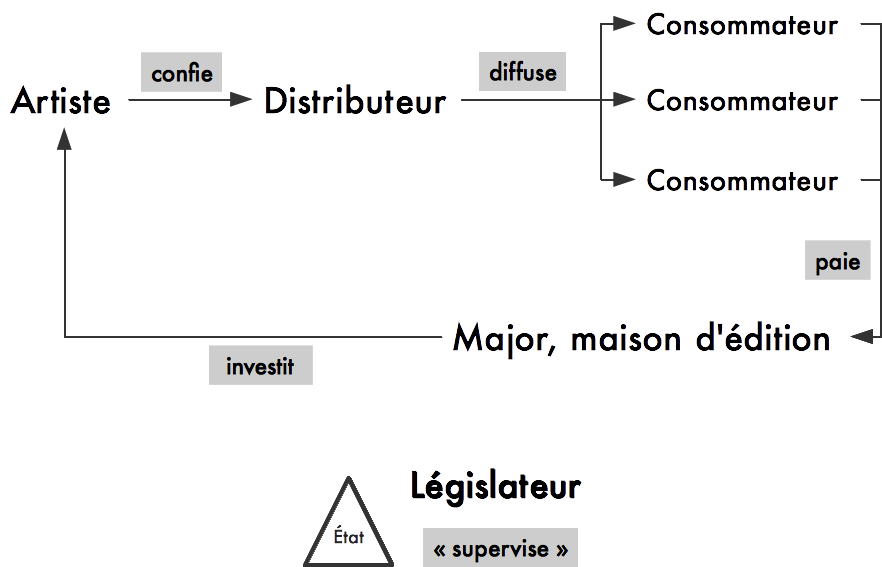
\includegraphics[width=13cm]{images/organisation-industrie-culturelle.png}
		\caption{Vue simplifiée de l'organisation de l'industrie culturelle}
	\end{figure}

	Au moment de sa forte croissance et de l'émergence des majors, l'industrie de la musique s'est organisée en un système bien réglé. Nous dépeignons une version simplifiée du parcours d'une œuvre quelconque : que l'on parle d'un morceau de musique, films, séries, livres, jeux vidéo ou logiciels, le schéma reste presque identique.\\

	Tout d'abord, l'artiste (ou bien le groupe) produit une œuvre. Pour vivre au jour le jour, ou bien pour couvrir les frais de production, l'artiste peut recevoir une avance sur les recettes futures de la part de sa maison d'édition ou d'une major. L'œuvre est ensuite confiée au distributeur, qui se charge de la vendre aux consommateurs finaux. Ces derniers paient le distributeur pour acquérir un exemplaire physique ou digital. Le distributeur reverse de l'argent à la major, qui en redistribue enfin une part à l'artiste original.\\

	Un des éléments-clés ici est le rôle de producteur qu'assument les majors. En effet, c'est grâce à cet investissement que de jeunes artistes peuvent tenter une percée dans le grand public. Cet investissement permet notamment de couvrir les frais d'enregistrement et de communication, qui auraient sinon étés rédhibitoires. Lorsque les majors se sentent financièrement fragiles, elles se replient en toute logique vers les investissements les plus sûrs. Ce sont donc les artistes les plus originaux ou ``risqués'' qui subissent le manque à gagner des majors.\\

	On remarque bien que les intérêts de chacun de ces acteurs diffèrent. Les majors et distributeurs sont des sociétés privées : elles visent avant tout une forte rentabilité. On peut supposer que l'artiste souhaite vivre de son travail et toucher un public le plus grand possible. Le consommateur veut écouter la musique de ses groupes préférés, suivre les séries qu'il aime, etc ; ceci instantanément et à moindre coût. Le législateur, quand à lui, veille à ce que le schéma soit respecté – plus globalement, il s'assure que l'économie reste active.

	\begin{figure}[ht]
		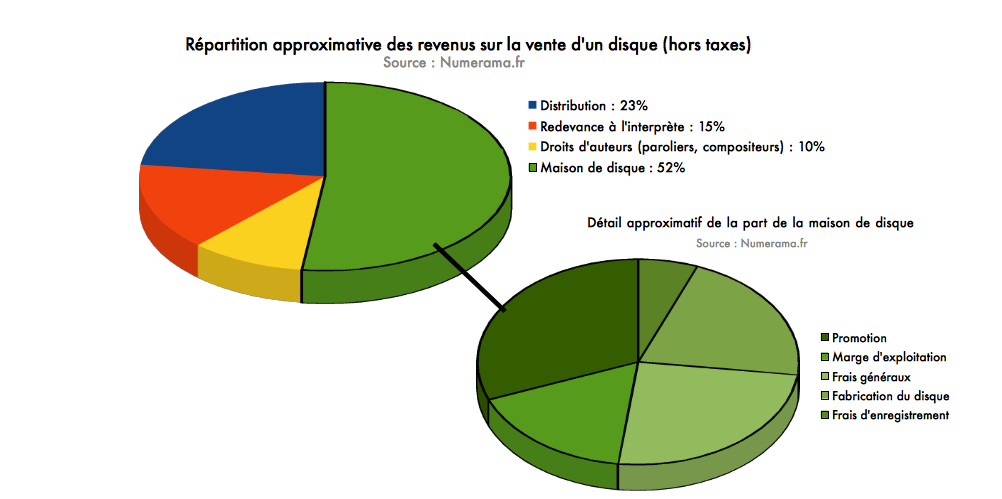
\includegraphics[width=13cm]{images/repartition-des-revenus.png}
		\caption{Répartition moyenne des revenus sur la vente d'un disque (hors taxes)}
	\end{figure}

	Il est important de remarquer qu'avec ce schéma d'organisation, les auteurs se partagent en général 10 à 15\% seulement du prix final payé par le consommateur\footnote{Hors taxes. Source : Epok, un hebdomadaire distribué par la FNAC.}. Ils peuvent cependant, dans une certaine mesure, s'appuyer sur d'autres sources de revenus : les diffusions à la radio ou à la télévision, les concerts, les locations, etc.
	% ------------------------------------ %

	% ------------------------------------ %
	% -- LA RÉVOLUTION NAPSTER ----------- %
	\section{La révolution Napster}
	Depuis l'avènement de l'Internet à haut-débit, la popularité du partage de fichiers est montée en flèche. D'abord réservée à un petit groupe de technophiles fréquentant les \emph{newsgroups}, cette pratique s'est rapidement étendue.

	\begin{figure}[ht]
		\begin{center}
			
\includegraphics[width=6cm]{images/logos/napster.jpg}
			\caption{Logo de Napster, le premier logiciel de partage \emph{peer-to-peer} populaire}
		\end{center}
	\end{figure}

	En Juin 1999, un véritable pavé est jeté dans la mare de l'industrie culturelle : Napster. Crée par Shawn Fanning et Sean Parker, ce logiciel basé sur la technologie \emph{peer-to-peer} permettait de partager facilement mais surtout gratuitement des fichiers de musique piratés. Son succès fulgurant poussa les majors à porter plainte pour violation massive du droit d'auteur, et le service fut fermé en juillet 2001\footnote{Source : Wikipédia [\href{http://fr.wikipedia.org/wiki/Napster}{fr.wikipedia.org/wiki/Napster}].}.\\

	Cependant, ce logiciel pionnier a inspiré la création de nombreux produits aux services similaires, dont une partie existe toujours : Emule, Limewire, Kazaa et Edonkey – pour ne citer que les plus connus. En effet, le service offert (partage de fichiers en utilisant la technologie \emph{peer-to-peer}) n'est pas illégal en soit, puisqu'il peut également servir à distribuer des fichiers libres de droits. Il s'agit par exemple d'un mode de transfert populaire pour les distributions Linux.

	% ------------------------------------ %
	% -- LE TÉLÉCHARGEMENT DIRECT -------- %
	\section{L'avènement du téléchargement direct}
	Depuis la mise en application de la loi Hadopi, qui prévoit la surveillance des réseaux P2P, les amateurs français de téléchargement se sont tournés\footnote{Source : comScore.} vers une solution alternative : le téléchargement direct. Cette technique, plutôt que de mettre à profit l'ensemble des téléchargeurs, établit une connexion directe avec un serveur, qui détient le fichier recherché. Ainsi, des hébergeurs de contenu tels que Mega.co.nz et Rapidshare fournissent les fichiers – souvent piratés – depuis leurs propres serveurs, situés dans des pays n'appliquant pas la réglementation française concernant le droit d'auteur. Bien que le téléchargement lui même soit gratuit pour l'utilisateur, ces entreprises sont financées par la publicité et proposent même un abonnement ``premium'' garantissant une vitesse de téléchargement plus élevée.\\

	Une dernière technologie a vu sa popularité exploser ces dernières années : le \emph{streaming}\footnote{Source : Google Trends.}. Elle permet à l'utilisateur de commencer à regarder une vidéo tout en la téléchargeant ; c'est donc l'outil parfait de consommation instantanée. Utilisée dans un cadre légal par Youtube, Dailymotion et d'autres services d'hébergement de vidéos, elle peut tout aussi bien servir au visionnage de longs-métrages. La démocratisation de son usage – facilitée par des annuaires de liens tels que Allostreaming – a provoqué un grand vent de panique dans l'industrie du cinéma.
	% ------------------------------------ %

	% ------------------------------------ %
	% -- POPCORN TIME -------------------- %
	\section{Popcorn Time, une vidéothèque \emph{peer-to-peer}}
	En avril 2014, l'industrie cinématrographique française rencontre deux nouvelles menaces. D'une part l'arrivée de Netflix — le géant américain du \emph{streaming} vidéo illimité sur abonnement — en France se précise, avec une date d'ouverture du service prévue pour ??? 2014  \cite{netflix-date-france} . D'autre part, une application, Popcorn Time  \cite{popcorn-time}, est publiée le ??? avril 2014. Elle fait rapidement parler d'elle et reçoit beaucoup d'attention dans les médias spécialisés \cite{popcorn-time-article}. Et pour cause : Popcorn Time pourrait bien devenir le Napster de la vidéo. En effet, cette application propose, tout comme Netflix, de regarder des films et séries en \emph{streaming}, immédiatement, via une interface très intuitive. Seule différence : le visionnage est gratuit, puisqu'il s'agit de films piratés, diffusés en \emph{peer-to-peer}. L'application est par ailleurs \emph{open-source} : son code est publié \cite{popcorn-time-github} et donc facilement distribuable. L'application étant développée par une communauté, les inévitables poursuites judiciaires à venir ne pourront pas porter sur un auteur en particulier. De plus, le caractère décentralisé du logiciel rend virtuellement impossible son blocage.
	% ------------------------------------ %

	% ------------------------------------ %
	% -- UN SYSTÈME SUR LE DÉCLIN -------- %
	\section{Un système sur le déclin}
	\label{declin-systeme}

	\begin{figure}[ht]
		\begin{center}
			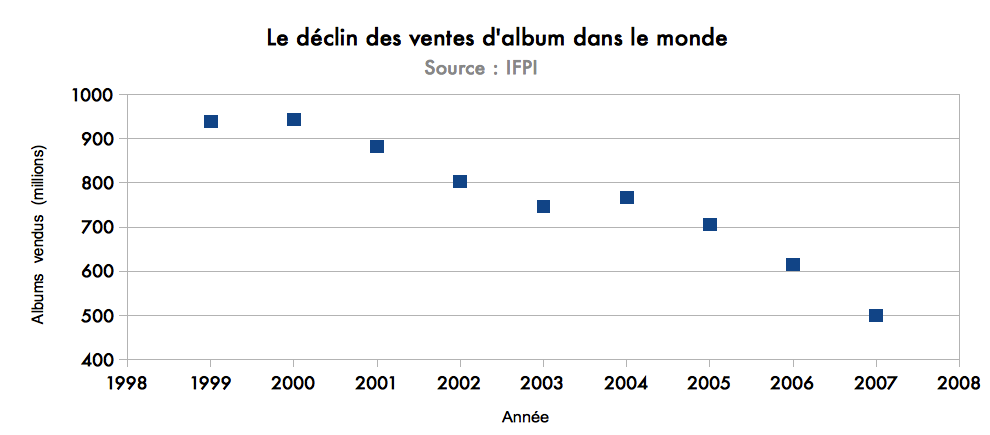
\includegraphics[width=10cm]{images/ventes-albums.png}
			\caption{Le déclin des ventes d'album dans le monde}
		\end{center}
	\end{figure}

	Depuis la banalisation du téléchargement illégal, les ventes de musique sur support physique n'ont cessé de chuter\footnote{Source : IFPI.}. Malgré l'explosion des ventes de musique dématérialisée, le marché reste en baisse. L'industrie du disque est en crise grave et peine à s'adapter aux nouveaux usages. 
	Également touchées, les ventes de DVD: entre 2005 et 2008, le marché français a enregistré une baisse de 30\%\footnote{Source : SEVN.}. Le contraire eut été étonnant : comment le DVD, payant et disponible seulement après six mois d'attente, pourrait se maintenir face à la concurrence du téléchargement illégal, gratuit et disponible parfois même avant la sortie en salles ?\\

	Force est de constater que l'adoption massive du téléchargement illégal a profondément modifié les habitudes des consommateurs. Les jeunes – ces \emph{digital natives} qui constitueront bientôt la majorité du public-cible de l'industrie culturelle – ne sont plus habitués à payer pour de la culture. Dans ce cadre, le schéma présenté plus tôt ne peut se maintenir. Deux alternatives s'ouvrent alors : tenter de ``rétablir l'ordre'' afin de maintenir l'organisation actuelle ou bien réviser ce système et l'adapter aux nouvelles contraintes.
	% ------------------------------------ %

	% ///////////////////////////////////////////////////////// %




	% ///////////////////////////////////////////////////////// %
	% /// LES MESURES EN APPLICATION ////////////////////////// %
	\chapter{Les mesures en application}

	% ------------------------------------ %
	% -- TENTATIVES DE RÉGULATION -------- %
	\section{Tentatives de régulation}

		\subsection{L'échec des DRM}
		Les verrous numériques constituent la première réponse technique apportée au problème du piratage. Le but premier est de limiter la copie des fichiers afin d'empêcher leur mise à disposition sur les réseaux de partage. Ainsi, un fichier de musique protégé par un verrou numérique (on parle de \emph{DRM}, Digital Rights Management) ne pourra être écouté que par la personne l'ayant acheté. De même, l'installation d'un logiciel commercial nécessite souvent une clé d'activation : cette clé ne peut être utilisée qu'un nombre défini de fois (en général trois à cinq fois), ce qui empêche le partage massif et limite les possibilités de prêt.\\

		En théorie, les DRM devaient régler le problème du téléchargement illégal par la suppression des sources. Mais en pratique, ces protections ont toujours été contournées rapidement par les plus ingénieux. Les produits initialement protégés sont donc finalement autant partagés que les autres une fois le verrou cassé. Apparaît alors un paradoxe : les clients ayant acheté une œuvre protégée par un tel verrou subissent les limites imposées par les DRM alors qu'une personne ayant piraté cette même œuvre disposera d'un fichier complètement libre.\\

		C'est ce constat qui a conduit à un recul de l'utilisation des verrous numériques. À l'initiative du plus grand magasin de musique digitale \emph{iTunes Store} en 2007 \cite{itunes-plus-release}, la plupart des marchands de musique en ligne ont abandonné cette méthode de protection. Aujourd'hui, les DRM appliqués à d'autres types de contenus sont encore décriés

		\subsection{Hadopi, une initiative française}
		La loi Hadopi, crée à l'initiative de la ministre de la Culture et de la Communication Christine Albanel, a été adoptée par le Sénat et l'Assemblée Nationale en mai 2009 \cite{hadopi-adoption}. Elle comporte deux volets : un volet visant à éduquer la population grâce à un dispositif de ``riposte graduée'' et un volet d'amélioration de l'offre légale. Les sanctions de la ``riposte graduée'' viennent s'ajouter à celles déjà prévues en matière de contrefaçon – jusqu'à trois ans de prison et 300 000\euro\ d'amende\footnote{Peines prévues par la loi DADVSI (loi relative au droit d’auteur et aux droits voisins dans la société de l’information).}.\\

		Techniquement, le dispositif Hadopi repose sur la surveillance de l'activité des réseaux \emph{peer-to-peer}. L'adresse IP des usagers téléchargeant certains fichiers surveillés (une liste d'environ 10 000 fichiers mise à jour régulièrement \cite{hadopi-fichiers-surveilles}) est consignée. À la première infraction, un message électronique est envoyé au contrevenant. Lorsqu'une deuxième infraction est repérée, c'est un courrier en recommandé qui parvient au domicile du téléchargeur. Enfin, si un troisième téléchargement illégal est détecté, la personne s'expose à des sanctions allant jusqu'à la coupure de l'accès à Internet pendant un an.\\

		La volonté d'améliorer l'offre légale s'est traduite par la création du label \emph{PUR} \cite{label-pur}, qui certifie les boutiques en ligne. L'utilisateur bénéficie ainsi d'un repère lorsqu'il souhaite se procurer musique et films en toute légalité.\\

		\label{hadopi-echec}
		Après ??? ans de fonctionnement, le bilan est mitigé. Avec ??? e-mails d'avertissement envoyés par jour, seule une condamnation a été prononcée : un ??? a écopé de 600\euro d'amende et 15 jours de suspension d'accès à Internet pour avoir téléchargé illégalement des morceaux de musique. Cependant, même cette unique peine n'a pas été appliquée. \cite{hadopi-condamnation}.

		TODO: graphique mode de téléchargement VS temps.

		On pourrait saluer la réussite de la mission éducative de l'Hadopi, puisque les chiffres du téléchargement \emph{peer-to-peer} en France montrent une baisse considérable. Il faut cependant prendre en compte le développement des nouveaux modes opératoires (téléchargement direct, streaming) décrits en première partie, dont la popularité ne peut être mesurée avec précision. Ces chiffres pourraient alors s'expliquer par un simple changement des habitudes des français.

		\subsection{SOPA/PIPA et ACTA}
		L'année 2011 et le début de 2012 ont été marqués par deux grands projets de loi portant sur le droit d'auteur.\\

		Aux États-Unis, le ``Stop Online Piracy Act'', proposé à la chambre des représentants – et son équivalent ``PROTECT IP''\footnote{Preventing Real Online Threats to Economic Creativity and Theft of Intellectual Property} proposé au sénat – visent tous deux à élargir les moyens disponibles pour la lutte contre le piratage et la contrefaçon. SOPA prévoit notamment des sanctions contre les sites donnant accès à du contenu protégé par le droit d'auteur. Ces sanctions s'étendent de la coupure des revenus publicitaires jusqu'au blocage complet. Ainsi, une procédure simplifiée serait mise à disposition des ayant-droits, leur permettant de faire fermer le site contrevenant sans faire appel à un juge. Les discussions concernant ces deux projets de lois ont été suspendues pour une durée indéterminée ``dans l'attente d'un accord'' \cite{suspension-sopa} suite aux nombreuses protestations, aux États-Unis comme à l'international.\\

		ACTA\footnote{Anti-Counterfeiting Trade Agreement}, quant à lui, est un traité international négocié avec 39 pays \cite{no-to-acta} depuis 2007. Il porte sur la propriété intellectuelle (notamment le respect du droit d'auteur sur Internet) et la contrefaçon. ACTA prévoyait de rendre responsable les fournisseurs d'accès internet (Orange, Free, etc) du comportement de leurs utilisateurs – leur donnant ainsi l'obligation de censurer leur propre réseau. Il a été signé par le comité exécutif de l'Union Européenne le 26 janvier 20125 malgré les remarques du parlement européen et les nombreuses manifestations à l'encontre de ce projet. Cependant, le projet de loi a été rejeté le 4 juillet 2012 par le Parlement européen \cite{acta-vote} à une large majorité\footnote{478 voix contre, 39 voix pour et 165 abstentions}.

	% ------------------------------------ %

	% ------------------------------------ %
	% -- DES COUPS DE FILET MÉDIATISÉS --- %
	\section{Des coups de filet médiatisés}
	Plusieurs des grandes entreprises victimes du piratage ont élaboré des processus de traitement des infractions au droit d'auteur. En réaction à la montée en flèche de l'utilisation du \emph{streaming}, les grands studios de production ont mis sur pied un plan de lutte contre ces nouveaux moyens de piratages \cite{lutte-streaming}. Faute de pouvoir faire fermer certains sites jugés illégaux hébergés à l'étranger, ce plan propose de bloquer l'accès au niveau des fournisseurs d'accès à internet. Le ``déréférencement'' de ces sites auprès des grands moteurs de recherche comme Google et Bing est également demandé. Unes des autres solutions régulièrement mise en avant est de bloquer leurs revenus publicitaires.\\

	Ces efforts ont abouti, en 2013, à deux grandes victoires : la fermeture de l'annuaire de lien Allostreaming \cite{allostreaming} et de l'hébergeur de fichiers Megaupload. Ce dernier a subi une fin médiatisée \cite{megaupload-fermeture} suite à un raid de police et une saisie des serveurs. Son fondateur, l'extravagant ``Kim Dotcom'', dénonce le préjudice porté aux utilisateurs légitimes du service, qui ont ainsi perdu accès à leurs données personnelles \cite{megaupload-prejudice}. Le procès est prévu pour ??? et devrait se baser sur des accusations de ??? et ??? \cite{megaupload-proces}.\\

	Mais, la demande restant fortement présente, et les barrières à l'entrée faibles, de nombreux services sont venus prendre leur place. En particulier, ``Kim Dotcom'' a mis sur pied le succeseur de Megaupload, qui a ouvert en ???. Cette fois, la légalité du service est assurée par le fait que toutes les données sont chiffrée côté client avant d'êtres envoyées vers les serveurs. Ainsi, l'hébergeur n'a aucune visibilité sur le contenu de ses utilisateurs.

	% ------------------------------------ %

	% ///////////////////////////////////////////////////////// %




	% ///////////////////////////////////////////////////////// %
	% /// PISTES ALTERNATIVES DE RÉSOLUTION /////////////////// %
	\chapter{Pistes alternatives de résolution}

	% ------------------------------------ %
	% -- DIVERSIFICATION DE L'OFFRE LÉGALE %
	\section{La diversification de l'offre légale comme alternative au piratage}
	Le secret de l'attractivité du téléchargement illégal tient en trois mots : gratuité, diversité, instantanéité. Le dernier point est particulièrement important : pour les films et séries, il est trop souvent impossible de les regarder légalement. En effet, jusqu'à récemment, la sortie en DVD d'un film avait lieu six mois après sa sortie en salle ; ce délai monte encore aujourd'hui jusqu'à un an pour ce qui est des séries étrangères, pourtant construites sur un modèle de diffusion hebdomadaire. Il semble alors que l'offre légale doit s'améliorer en priorité sur ces trois critères pour pouvoir faire face au téléchargement illégal.\\

	Comme souligné par Pascal Nègre\footnote{Président Directeur Général d'Universal Music France} dans \cite{podcast-industrie-musicale}, l'industrie musicale est la première a avoir ``accompli sa révolution complète''. En effet, le prix de 0,99\euro\ par titre, la facilité d'achat et la grande disponibilité internationale des morceaux font du monde musical le plus avancé dans le domaine du numérique. De plus, l'abandon des verrous numériques est synonyme de réelle propriété pour le consommateur : il est libre de copier, sauvegarder, écouter où il le souhaite et éventuellement partager le fichier dont il a fait l'acquisition.\\

	De même, l'offre dématérialisée en termes de jeux vidéo est très fournie. La plupart des jeux sortent désormais simultanément en boutiques et sur des plate-formes comme Steam. Du côté de la vidéo cependant, le constat est moins probant. Quelques initiatives présagent tout de même une amélioration : le délai de disponibilité des films à la demande (VOD) a été légalement fixé à quatre mois maximum \footnote{Source : SEVN}. Plusieurs chaînes françaises (\emph{TF1 Vision}, \emph{Orange Cinéma Séries}) donne quant à elles accès aux derniers épisodes de quelques séries américaines le lendemain de leur première diffusion – et donc au même niveau d'instantanéité que le téléchargement illégal.\\

	Un autre mode de consommation, très populaire\footnote{Selon \emph{Sandvine}, le service de vidéo sur demande \emph{Netflix} représente plus de 30\% du trafic Internet aux États-Unis.} pour les films aux États-Unis, est l'abonnement illimité. Pour 8\$ par mois, la société \emph{Netflix} propose un accès illimité et instantané à tout son catalogue de films et de séries grâce en \emph{streaming}.\\

	En France, \emph{Deezer} propose un service similaire dans le domaine musical : pour 10\euro\ par mois, tout le catalogue est accessible, y compris sur les appareils mobiles. Comme l'utilisateur ne fait que consulter des œuvres stockées chez le fournisseur et ne garde aucune copie sur sa machine, il souscrit effectivement à un service d'accès, et non plus pour être propriétaire d'une copie privée. Dans \cite{podcast-industrie-musicale}, Pascal Nègre, en défense des supports physiques, remarque que de tels services ne répondent pas au ``besoin naturel de collectionner'' ressenti, d'après lui, par tout un chacun.\\

	Ce type d'offres est le seul à offrir un confort comparable à celui du piratage : une fois l'abonnement payé, l'accès est ``gratuit'', illimité et immédiat, ce qui explique sa popularité croissante.

	\begin{figure}[ht]
		\begin{center}
			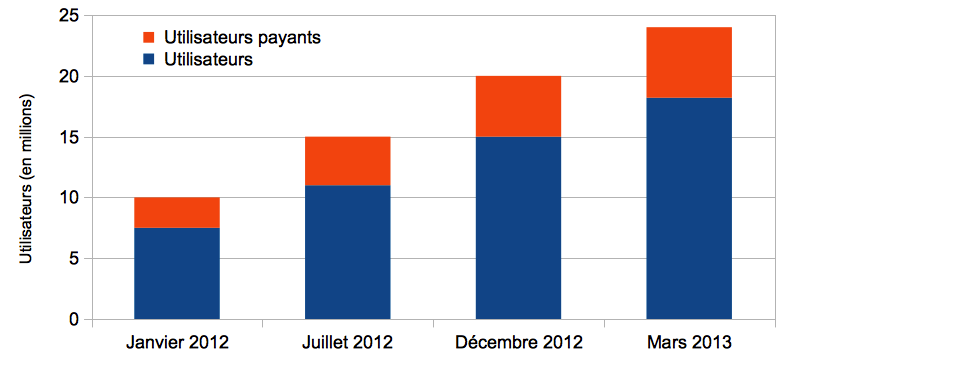
\includegraphics[width=14cm]{images/spotify-croissance.png}
			\caption{Croissance du service Spotify (source CNET)}
		\end{center}
	\end{figure}

	Cependant, il est important de garder à l'esprit que ces services ne peuvent exister qu'à condition que les majors acceptent rendre disponible leur catalogue \cite{podcast-industrie-musicale}.
	% ------------------------------------ %

	% ------------------------------------ %
	% -- LA DISTRIBUTION DIRECTE --------- %
	\section{La distribution directe}
	Le ``milieu indépendant'' peut être source d'idées novatrices. Qu'il s'agisse de groupes de musiques ou de petits studios de développement de jeu vidéo, leur échelle réduite leur permet d'expérimenter de nouveaux modes de distribution.\\

	Le groupe \emph{Radiohead} a par exemple choisi de rendre le paiement de son album \emph{In Rainbows} optionnel \cite{radiohead}, à l'image d'un concert gratuit où l'on ferait passer le chapeau : on donne si l'on a aimé et si l'on en a les moyens.\\

	Une initiative similaire a lieu de manière périodique dans le monde du jeu vidéo depuis mai 2010 : le \emph{Humble Indie Bundle} \cite{humble-indie-bundle}. Le principe est simple : proposer pendant une courte période un pack de plusieurs jeux produits par des studios indépendants à un prix déterminé par l'acheteur. Ce dernier peut également profiter de son achat pour faire un don à des associations caritatives. De plus, un mécanisme ingénieux a été mis en place : en payant plus que la moyenne, l'acheteur gagne le droit de télécharger la bande-son des jeux proposés, voire l'ensemble des jeux de l'édition précédente. Depuis le lancement, ce sont près de 80 millions de dollars qui auront été remportés \cite{humble-stats}.\\

	Il s'agit dans les deux cas de modèles tirant parti des avantages de la distribution directe dématérialisée : les créateurs sont à la fois artistes et distributeurs, ils établissent une relation directe avec le consommateur. En écartant les intermédiaires, la rémunération de l'artiste est bien plus conséquente.

	Cependant, avec ce modèle de distribution à bas prix, on est en droit de se poser la question de la pérennité. L'énorme volume de vente amène l’œuvre à rencontrer un grand public, et apporte donc une notoriété immédiate à ses créateurs. Mais ce public ne risque-t-il pas justement de perdre l'habitude de payer un prix ``normal'' ? D'après \cite{low-prices-low-expectations}, cette érosion des prix comporte un grand risque : celui de dévaluer la qualité des œuvres proposées.
	% ------------------------------------ %

	% ------------------------------------ %
	% -- LA PRODUCTION COMMUNAUTAIRE ----- %
	\section{La production communautaire}
	

	% ------------------------------------ %

	% ------------------------------------ %
	% -- PARTICIPATION DE L'ÉTAT --------- %
	\section{Vers une participation accrue de l'État ?}
	Dans le schéma présenté en première partie, le rôle du ``législateur'' est de s'assurer du bon développement de l'économie de la culture. Mais, en la personne de l'État, sa position ne pourrait-elle pas devenir plus active ?\\

	Le gouvernement français a pris pour devoir l'éducation vis à vis des problématiques du droit d'auteur. L'Hadopi a ainsi lancé en juin 2011 une campagne de publicité multi-supports (télévision, Internet, affiches, radio). La Haute Instance n'ayant conduit qu'à une seule condamnation, elle est d'ailleurs maintenant décrite par ses défenseurs comme un dispositif ``avant tout pédagogique'' \cite{podcast-industrie-musicale}.\\

	Autre opération, lancée par le Ministère de la Culture : la Carte Musique Jeune. Lancée en 2010, elle proposait aux 12-25 ans un financement à hauteur de 50\% sur leurs achats de musique digitale (dans la limite de 50\euro par an et par personne). Cette réduction était disponible auprès quatorze marchands partenaires dont l'iTunes Store ; mais la carte permettait aussi de s'abonner à la formule d'écoute illimitée chez Deezer. De quoi inciter certains à rentrer dans un cadre légal. Cependant, le dispositif a été considéré comme un échec \cite{carte-musique-jeune-echec} et a été retiré en octobre 2012 \cite{carte-musique-jeune-arret}.\\

	La modification profonde de l'économie de la culture par l'arrivée d'Internet demande une réponse politique plus forte. Les solutions actuelles au téléchargement illégal, basées sur le blocage ou la surveillance, se révèlent soit inefficaces car contournées, soit liberticides. En effet, le filtrage proposé dans les projets ACTA et SOPA/PIPA, représente une porte ouverte à une censure facilitée de la part des gouvernements et d'entreprises privées \cite{quadrature-filtrage}.\\

	François Hollande, dans son programme pour les élections présidentielles de 2012, proposait de rendre possible la dépénalisation du téléchargement par le biais d'une ``licence globale''. Il s'agirait de taxer les abonnements à Internet et la publicité en ligne – comme c'est déjà le cas pour les supports vierges – afin de rémunérer les artistes \cite{licence-gloable}. L'idée a été citée à nouveau à quelques occasions, mais les détails manquent : ces taxes couvriront-elles réellement le manque à gagner induit par le piratage ? Comment répartir ces nouveaux revenus entre les artistes ? Comment rendre cette solution adaptée pour un marché maintenant global ?\\

	Malgré toute ces interrogations, l'idée d'un ``forfait'' semble malgré toujours plus réaliste que la mise en place d'un blocage réussissant à être à la fois véritablement efficace et respectueux des libertés fondamentales des internautes.
	% ------------------------------------ %

	% ///////////////////////////////////////////////////////// %




	% ///////////////////////////////////////////////////////// %
	% /// CONCLUSION ////////////////////////////////////////// %
	\chapter{Conclusion}

	Bye.
	% ///////////////////////////////////////////////////////// %



	% Génération de la page de garde
	\bibliographystyle{bibstyle}
	\bibliography{references}




% Fin du document
\end{document}